% Source: graduate-coursework/Prior_Semesters/Sp24/EMCH354/assignments/HW2/HW2.tex

\documentclass[border=4pt]{standalone}
\usepackage{amsmath}
\usepackage{tikz}
\usetikzlibrary{patterns}
\usetikzlibrary{arrows.meta, decorations.pathmorphing}

\definecolor{bluecolor}{RGB}{173,216,230}
\definecolor{purplecolor}{RGB}{210,180,222}
\definecolor{pinkcolor}{RGB}{255,182,193}
\definecolor{orangecolor}{RGB}{252, 213, 180}

\begin{document}
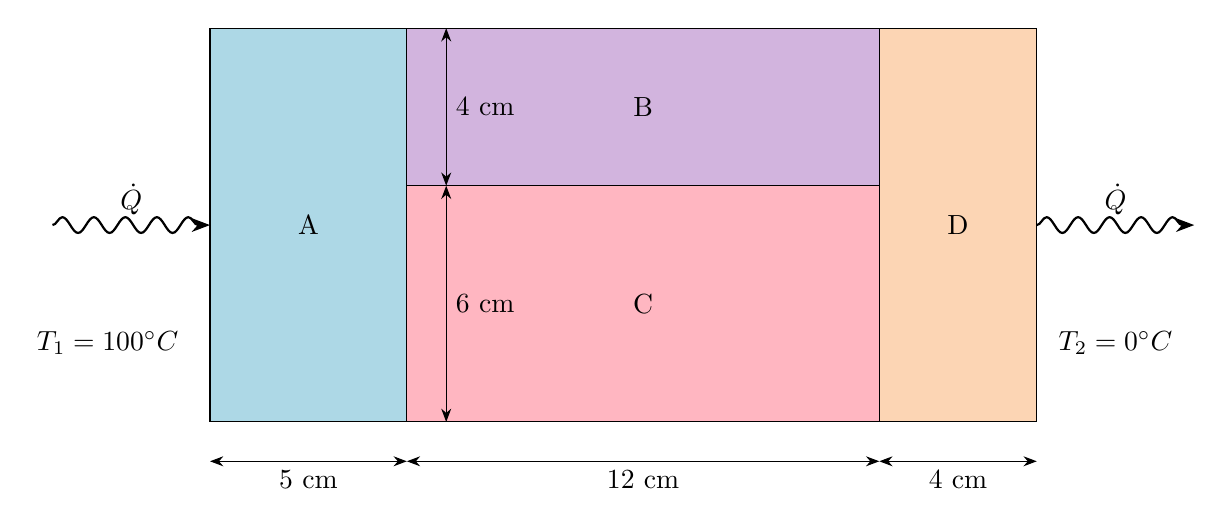
\begin{tikzpicture}[scale=0.5, >=Stealth]
% Define nodes for the temperatures
\node (T1) at (-2.6,2) {\(T_1 = 100^\circ C\)};
\node (T2) at (23,2) {\(T_2 = 0^\circ C\)};

% Draw the composite wall
\draw[fill=bluecolor] (0,0) rectangle (5,10); % Material A
\draw[fill=purplecolor] (5,6) rectangle (17,10); % Material B
\draw[fill=pinkcolor] (5,0) rectangle (17,6); % Material C
\draw[fill=orangecolor] (17,0) rectangle (21,10); % Material D

% Labels for materials
\node at (2.5,5) {A};
\node at (11,8) {B};
\node at (11,3) {C};
\node at (19,5) {D};

% Dimensions
\draw[<->] (0,-1) -- node[below] {5 cm} (5,-1);
\draw[<->] (5,-1) -- node[below] {12 cm} (17,-1);
\draw[<->] (17,-1) -- node[below] {4 cm} (21,-1);
\draw[<->] (6,6) -- node[right] {4 cm} (6,10);
\draw[<->] (6,0) -- node[right] {6 cm} (6,6);

% Heat flow arrows
\draw[->, thick, decorate, decoration={snake, amplitude=1mm, segment length=4mm, post length=1mm}] (-4,5) -- (0,5) node[midway,above] {\(\dot{Q}\)};
\draw[->, thick, decorate, decoration={snake, amplitude=1mm, segment length=4mm, post length=1mm}] (21,5) -- (25,5) node[midway,above] {\(\dot{Q}\)};
\end{tikzpicture}
\end{document}
